\chapter{Bayesian Statistic}

\section{Statistic v.s. Probability}
Statistics focuses on real-life applications where the underlying distribution is often unknown. To address this, we use \textbf{statistical inference} to analyze observed data and estimate the unknown distribution. Rather than finding the exact distribution, we approximate it using models such as parametric (e.g., normal, exponential) or non-parametric approaches. Once a suitable model is chosen, probability laws help us make predictions and draw conclusions, though these approximations involve assumptions and uncertainties.  

Now, let's move on to our first topic in statistics: 

\section{Bayesian Statistics}

\subsection{Introduction}
In the probability course, we learned Bayes' Rule \href{https://ryanc.wtf/files/ENGG2760.pdf#page=14}{ENGG2760: Theorem 3.2.1}, which helps us calculate conditional probabilities and, at times, update our beliefs based on new evidence.

And it turns out that one of the statistical inferences we use is based on Bayes' rule, namely Bayesian statistical inference. In Bayesian statistical inference, we: (1) assign prior probabilities to parameters; (2) observe data; and (3) update probabilities via Bayes' rule:
\[
  \underbrace{f_{\Theta \vert X} (\theta \vert x)}_{\text{Posterior}} = \dfrac{\overbrace{f_{\Theta} (\theta)}^{\text{Prior}} \overbrace{f_{X \vert \Theta} (x \vert \theta)}^{\text{Observation}}}{f_X (x)}
\]
Here we have both the posterior and prior probabilities of the parameters \(\theta\)  and observations \(x\).  

We have four variations of the Bayes' rule shown above.

\begin{table}[H]
  \centering
  \begin{tabular}{c|c}
      \toprule
      Condition & Bayes' rule  \\
    \midrule
      \(\Theta\) discrete, \(X\) discrete & \(p_{\Theta \vert X} (\theta \vert x) = \dfrac{p_{\Theta} (\theta) p_{X \vert \Theta} (x \vert \theta)}{\sum_{\theta^{\prime}} p_{\Theta} (\theta^{\prime}) p_{X \vert \Theta} (x \vert \theta^{\prime})}\)  \\
      \(\Theta\) discrete, \(X\) continuous & \(p_{\Theta \vert X} (\theta \vert x) = \dfrac{p_{\Theta} (\theta) f_{X \vert \Theta} (x \vert \theta)}{\sum_{\theta^{\prime}} p_{\Theta} (\theta^{\prime}) f_{X \vert \Theta} (x \vert \theta^{\prime})}\)  \\
      \(\Theta\) continuous, \(X\) discrete & \(f_{\Theta \vert X} (\theta \vert x) = \dfrac{f_{\Theta} (\theta) p_{X \vert \Theta} (x \vert \theta)}{\int f_{\Theta} (\theta^{\prime}) p_{X \vert \Theta} (x \vert \theta^{\prime})}\)  \\
      \(\Theta\) continuous, \(X\) continuous & \(f_{\Theta \vert X} (\theta \vert x) = \dfrac{f_{\Theta} (\theta) f_{X \vert \Theta} (x \vert \theta)}{\int f_{\Theta} (\theta^{\prime}) f_{X \vert \Theta} (x \vert \theta^{\prime})}\)  \\
      \bottomrule
  \end{tabular}
\end{table}

We can use \(Z(x)\) to denote the denominator for both discrete and continuous cases. It depends only on the observed data \(x\).

\begin{eg}[Probability Review]
  We flip a coin. How likely is it to get 2 heads in 3 coin flips if the probability of heads is \(p\), where \(p\) could be 0.5, 0.7, and 1? 
  
  Also, use the Central Limit Theorem to estimate the probability of at least 200 heads in 300 coin flips.

  \textbf{Solution:} 
  \[
    \mathbb{P}(H = 2) = \binom{3}{2} p^2(1 - p)
  \]
  \(p = 0.5: \mathbb{P}(H = 2) = \binom{3}{2} \times 0.5^2 \times 0.5 = 0.375\)

  \(p = 0.7: \mathbb{P}(H = 2) = \binom{3}{2} \times 0.7^2 \times 0.3 = 0.441\)

  \(p = 1: \mathbb{P}(H = 2) = \binom{3}{2} \times 1^2 \times 0 = 0\)

  For the probability of at least 200 heads in 300 coin-flips, 
  \[
    \text{H} \sim \text{Binomial}(300, p),\quad \mu = 300p,\quad \sigma = \sqrt{300p(1 - p)}
  \]
  \(p = 0.5: \mu = 150, \sigma = 8.66\)

  \(
  \begin{aligned}
    \mathbb{P}(H \geq 200) &= \mathbb{P}(\dfrac{H - 150}{8.66} \geq \dfrac{200 - 150}{8.66}) \\
    &= \mathbb{P}(z \geq 5.77) \\
    &\approx 0
  \end{aligned}
  \) 

  \(p = 0.7: \mu = 210, \sigma = 7.94\)

  \(
  \begin{aligned}
    \mathbb{P}(H \geq 200) &= \mathbb{P}(\dfrac{H - 210}{7.94} \geq \dfrac{200 - 210}{7.94}) \\
    &= \mathbb{P}(z \geq -1.26) \\
    &= \varPhi (1.26) \\
    &= 0.896
  \end{aligned}
  \) 
  
\end{eg}

Again, we flip a coin three times and get two heads. You are told that there are three types of coins with different priors, but you don’t know which coin you are flipping. It is obvious that the first coin flip will affect your belief (prior) about which coin you have. For example, if you see 100 heads out of 100 flips, you might strongly believe that both sides of the coin are heads. But to what extent does each flip influence your belief? This brings us to the problem of statistics.

\begin{eg}
  A coin can be one of three types:

  1. A fair coin \(\theta = 1\) with one head and one tail – 90\%

  2. A coin \(\theta = 2\) with both sides as heads – 5\%
  
  3. A coin \(\theta = 3\) with both sides as tails – 5\%

  Now, you flip a head without knowing which coin you have. How should you update your belief (priors)?

  \textbf{Solution:} 

  \(
  \begin{aligned}
    \mathbb{P}(\theta = 1 \vert H_1) &= \dfrac{\mathbb{P}(H_1 \vert \theta = 1)\mathbb{P}(\theta = 1)}{Z(H_1)} = \dfrac{0.5 \times 0.9}{Z(H_1)} = \dfrac{0.45}{Z(H_1)} \\
    \mathbb{P}(\theta = 2 \vert H_1) &= \dfrac{\mathbb{P}(H_1 \vert \theta = 2)\mathbb{P}(\theta = 2)}{Z(H_1)} = \dfrac{1 \times 0.05}{Z(H_1)} = \dfrac{0.05}{Z(H_1)} \\
    \mathbb{P}(\theta = 3 \vert H_1) &= 0 \\
  \end{aligned}
  \) 

  Then we have \(\mathbb{P}(H_1) = Z(H_1) = 0.45 + 0.05 + 0 = 0.5\) 
  \[
    \mathbb{P}(\theta = 1 \vert H_1) = \dfrac{0.45}{Z(H_1)} = 0.9 \quad \mathbb{P}(\theta = 1 \vert H_1) = \dfrac{0.05}{Z(H_1)} = 0.1 \quad \mathbb{P}(\theta = 1 \vert H_1) = 0
  \]

  From this, we can update our belief, which we can then use to further readjust our belief if the second flip also results in a head. 

  \(
  \begin{aligned}
    \mathbb{P}(\theta = 1 \vert H_2 H_1) &= \dfrac{\mathbb{P}(H_2 \vert \theta = 1, H_1)\mathbb{P}(\theta = 1 \vert H_1)}{Z(H_2, H_1)} = \dfrac{0.5 \times 0.9}{Z(H_2, H_1)} = \dfrac{0.45}{Z(H_2, H_1)} \\
    \mathbb{P}(\theta = 2 \vert H_2 H_1) &= \dfrac{\mathbb{P}(H_2 \vert \theta = 2, H_1)\mathbb{P}(\theta = 2 \vert H_1)}{Z(H_2, H_1)} = \dfrac{1 \times 0.1}{Z(H_2, H_1)} = \dfrac{0.1}{Z(H_2, H_1)} \\
    \mathbb{P}(\theta = 3 \vert H_2 H_1) &= 0 \\
  \end{aligned}
  \) 

  Then we have \(\mathbb{P}(H_2 H_1) = Z(H_2 H_1) = 0.45 + 0.01 + 0 = 0.55\) 
  \[
    \mathbb{P}(\theta = 1 \vert H_2 H_1) = \dfrac{0.45}{Z(H_2 H_1)} = 0.82 \quad \mathbb{P}(\theta = 1 \vert H_2 H_1) = \dfrac{0.1}{Z(H_2 H_1)} = 0.18 \quad \mathbb{P}(\theta = 1 \vert H_2 H_1) = 0
  \]
\end{eg}

% L01 finished
\subsection{Bayesian Statistical Inference}
For Bayesian statistics, we have only one formula: Bayes’s rule: 
\[
  \underbrace{f_{\Theta \vert X} (\theta \vert x)}_{\text{posterior}} \propto \underbrace{f_{X \vert \Theta} (x \vert \theta)}_{\text{likelihood}} \underbrace{f_{\Theta} (\theta)}_{\text{prior}}
\]

We have some prior knowledge, and after observing something, we can use the prior and likelihood to update our belief, which gives us the posterior. This posterior can later serve as the prior for another observation, allowing us to continuously update our belief throughout the observation process.

\begin{eg}
  Romeo is waiting for Juliet on their first date. He wants to estimate how long he will have to wait for her. Given that Romeo has some prior dating experience, he already has some prior knowledge about how late girls tend to be.
  
  Girl A - \(X \sim \text{Uniform}(0, 0.3)\); 
  
  Girl B - \(X \sim \text{Uniform}(0, 0.8)\); 

  Girl C - \(X \sim \text{Uniform}(0, 0.6)\), 

  where the uniform random variable shows the range of lateness. For example, for girl A, she will be late between the dating time and the dating time plus 0.3 hours. Then, how could you use Bayesian statistics to estimate the waiting time for Romeo's new girlfriend? 

  \textbf{Solution:} 
  Here we can set up the uniform random variable \(\text{Uniform}(0, \Theta)\), where \(\Theta\) depends on the girls' decision. Then what we need to find is the \(\theta\) for Juliet. We can then have 
  \[
    f_{X \vert \Theta}(x \vert \theta) = \begin{dcases}
      \frac{1}{\theta}, &\text{ if } 0 \leq x \leq \theta ;\\
      0, &\text{ otherwise} .
    \end{dcases}
  \]

  In Romeo's model, \(\theta\) is also a uniform random variable \(\theta \sim \text{Uniform}(0, 1)\), where \(X \sim \text{Uniform}(0, \Theta)\). Given that on their first date, Juliet arrived \(\frac{1}{2}\) hours late, we have 
  \[
    f_{\Theta \vert X} (\theta \vert \dfrac{1}{2}) \propto f_\Theta (\theta) f_{X \vert \Theta}(\dfrac{1}{2} \vert \theta) = \dfrac{1}{\theta}
  \]
  Here we have the prior \(f_\Theta(\theta) = 1\) if \(0 \leq \theta \leq 1\), and the likelihood \(f_{X \vert \Theta} (\frac{1}{2} \vert \theta) = \frac{1}{\theta}\) if \(\frac{1}{2} \leq \theta \leq 1\). Keep in mind that the prior comes from Romeo's model, where he has never dated a girl who is late for more than 1 hour, and it may not be valid if \(\theta > 1\), which shows the limitation of Bayesian statistics. Also, the observation (likelihood) shows the probability of Juliet arriving precisely at (or within a very small interval around) time plus 0.5. Therefore, we have \(\theta \geq \frac{1}{2}\). 

  For the integral to be equal to 1, we need to find the constant term. This can be found using calculus: 
  \[
    \int_\frac{1}{2} ^1 \dfrac{1}{\theta} d \theta= \ln \theta \Big|_{\frac{1}{2}}^1 = \ln 2 \Longrightarrow f_{\Theta \vert X} (\theta \vert \dfrac{1}{2}) = \dfrac{1}{\theta \ln 2}
  \]

  \begin{minipage}{0.5\textwidth}
    Here we have \(\theta < \frac{1}{2} = 0\) because from the data, we know that \(\theta \geq \frac{1}{2}\), which means the lateness parameter is at least \(\frac{1}{2}\), so it is not possible for Juliet to arrive between the dating time and dating time plus 0.5. We also have \(\theta > 1 = 0\) because from Romeo's prior knowledge, he knows that a girl would not be later than 1 hour.
  \end{minipage}
  \begin{minipage}{0.5\textwidth}
    \centering
    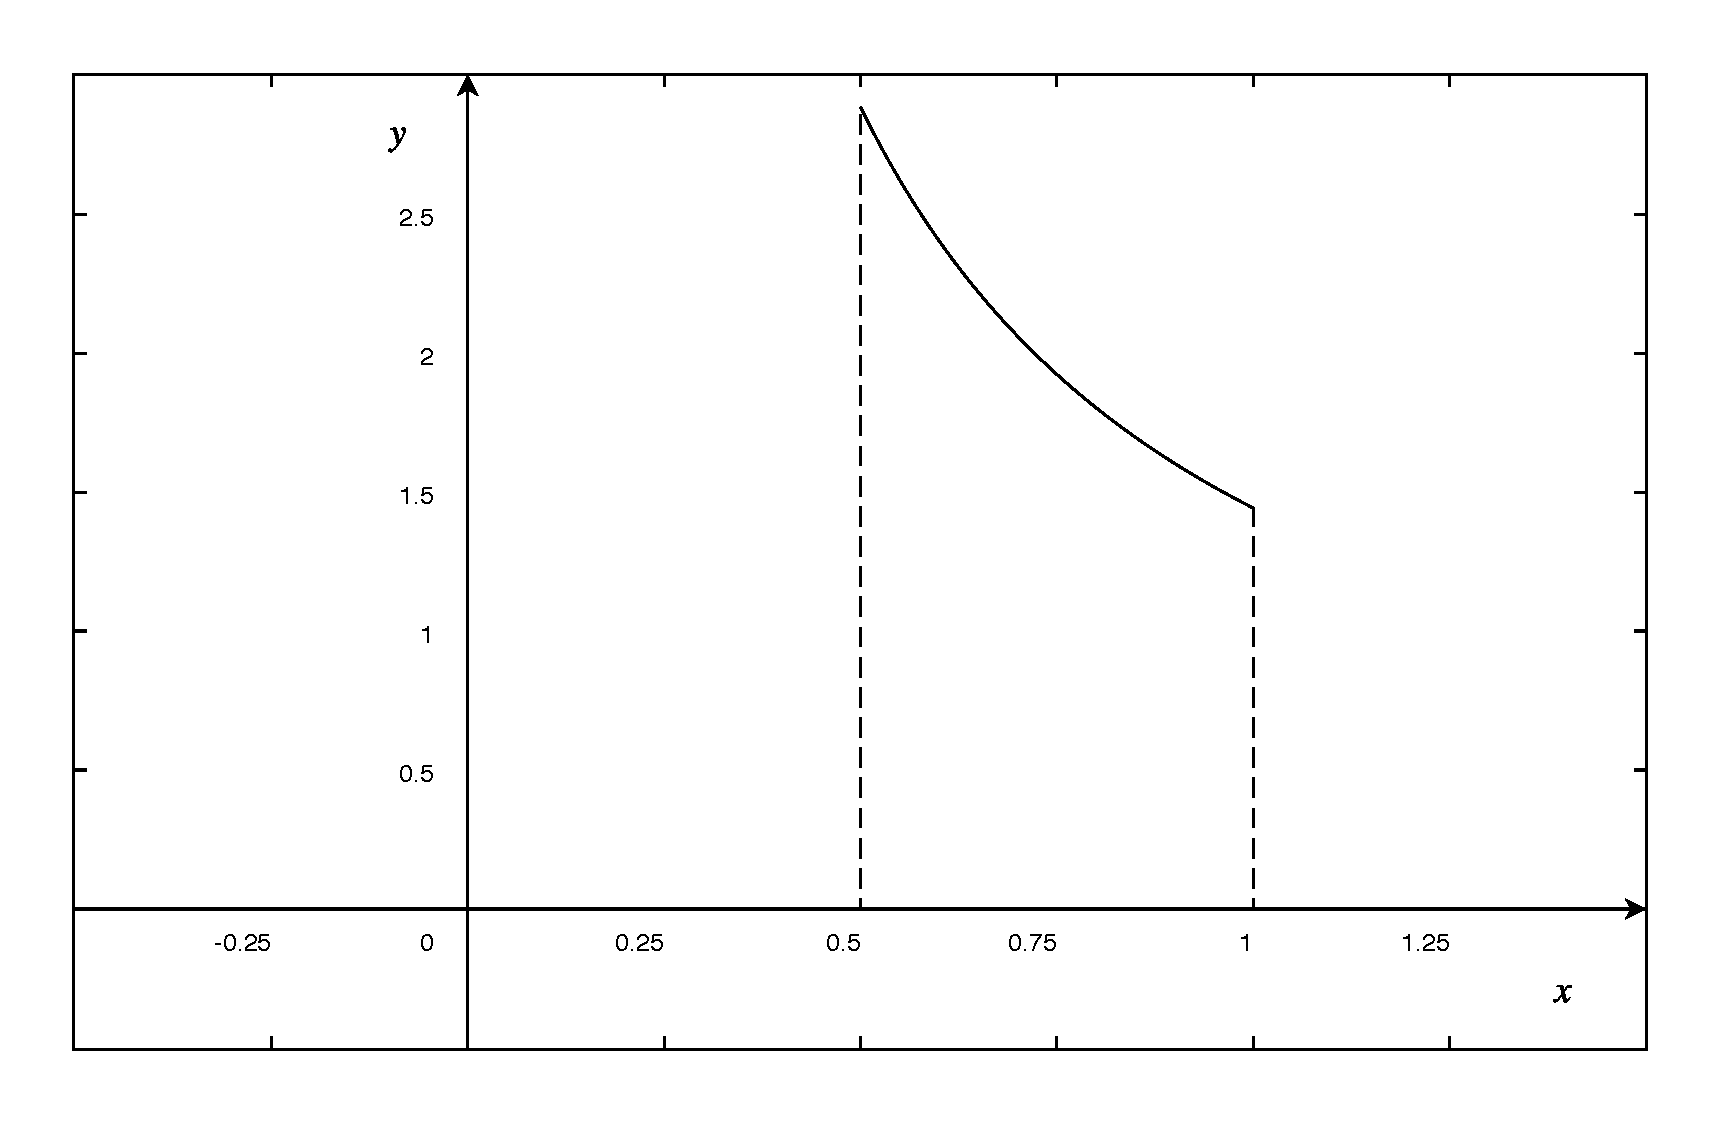
\includegraphics[width=0.8\textwidth]{Figures/Romeo_model.pdf}
  \end{minipage}

  On their second date, Juliet arrived \(\frac{1}{4}\) hours late. We then need to readjust the prior based on the previous model to find the new posterior.
  \[
    f_{\Theta \vert X_1, X_2} \left(\theta \Big| \dfrac{1}{2}, \dfrac{1}{4}\right) \propto f_{\Theta \vert X_1} \left(\theta \Big| \dfrac{1}{2}\right) f_{X_2 \vert \Theta, X_1}\left(\dfrac{1}{4} \Big| \theta, \frac{1}{2}\right)
  \]
  Here, since \(X_1\) and \(X_2\) are independent, we can discard \(X_1\) in the calculation.
  \[
    f_{\Theta \vert X_1, X_2} \left(\theta \Big| \dfrac{1}{2}, \dfrac{1}{4}\right) \propto f_{\Theta \vert X_1} \left(\theta \Big| \dfrac{1}{2}\right) f_{X_2 \vert \Theta}\left(\dfrac{1}{4} \Big| \theta\right) = \dfrac{1}{\theta \ln 2} \times \dfrac{1}{\theta} = \dfrac{1}{\theta^{2} \ln{(2)}} \propto \dfrac{1}{\theta^2}
  \]
  The same as above, we have \(f_{X_2 \vert \Theta} (\frac{1}{4} \vert \theta) = \frac{1}{\theta}\) since it is not possible for the lateness to be less than \(\frac{1}{4}\) hours. Also, given the prior as calculated in the first part, we have \(f_{\Theta \vert X_1} (\theta \vert \frac{1}{2}) = \frac{1}{\theta \ln 2}\) if \(\frac{1}{2} \leq \theta \leq 1\).

  For the integral to be equal to 1, we need to find the constant term. This can be found using calculus: 
  \[
    \int_\frac{1}{2} ^1 \dfrac{1}{\theta^2} d \theta = 1 \Longrightarrow f_{\Theta \vert X_1, X_2} \left(\theta \Big| \dfrac{1}{2}, \dfrac{1}{4}\right) = \dfrac{1}{\theta^2}
  \]

  \begin{figure}[H]
    \centering
    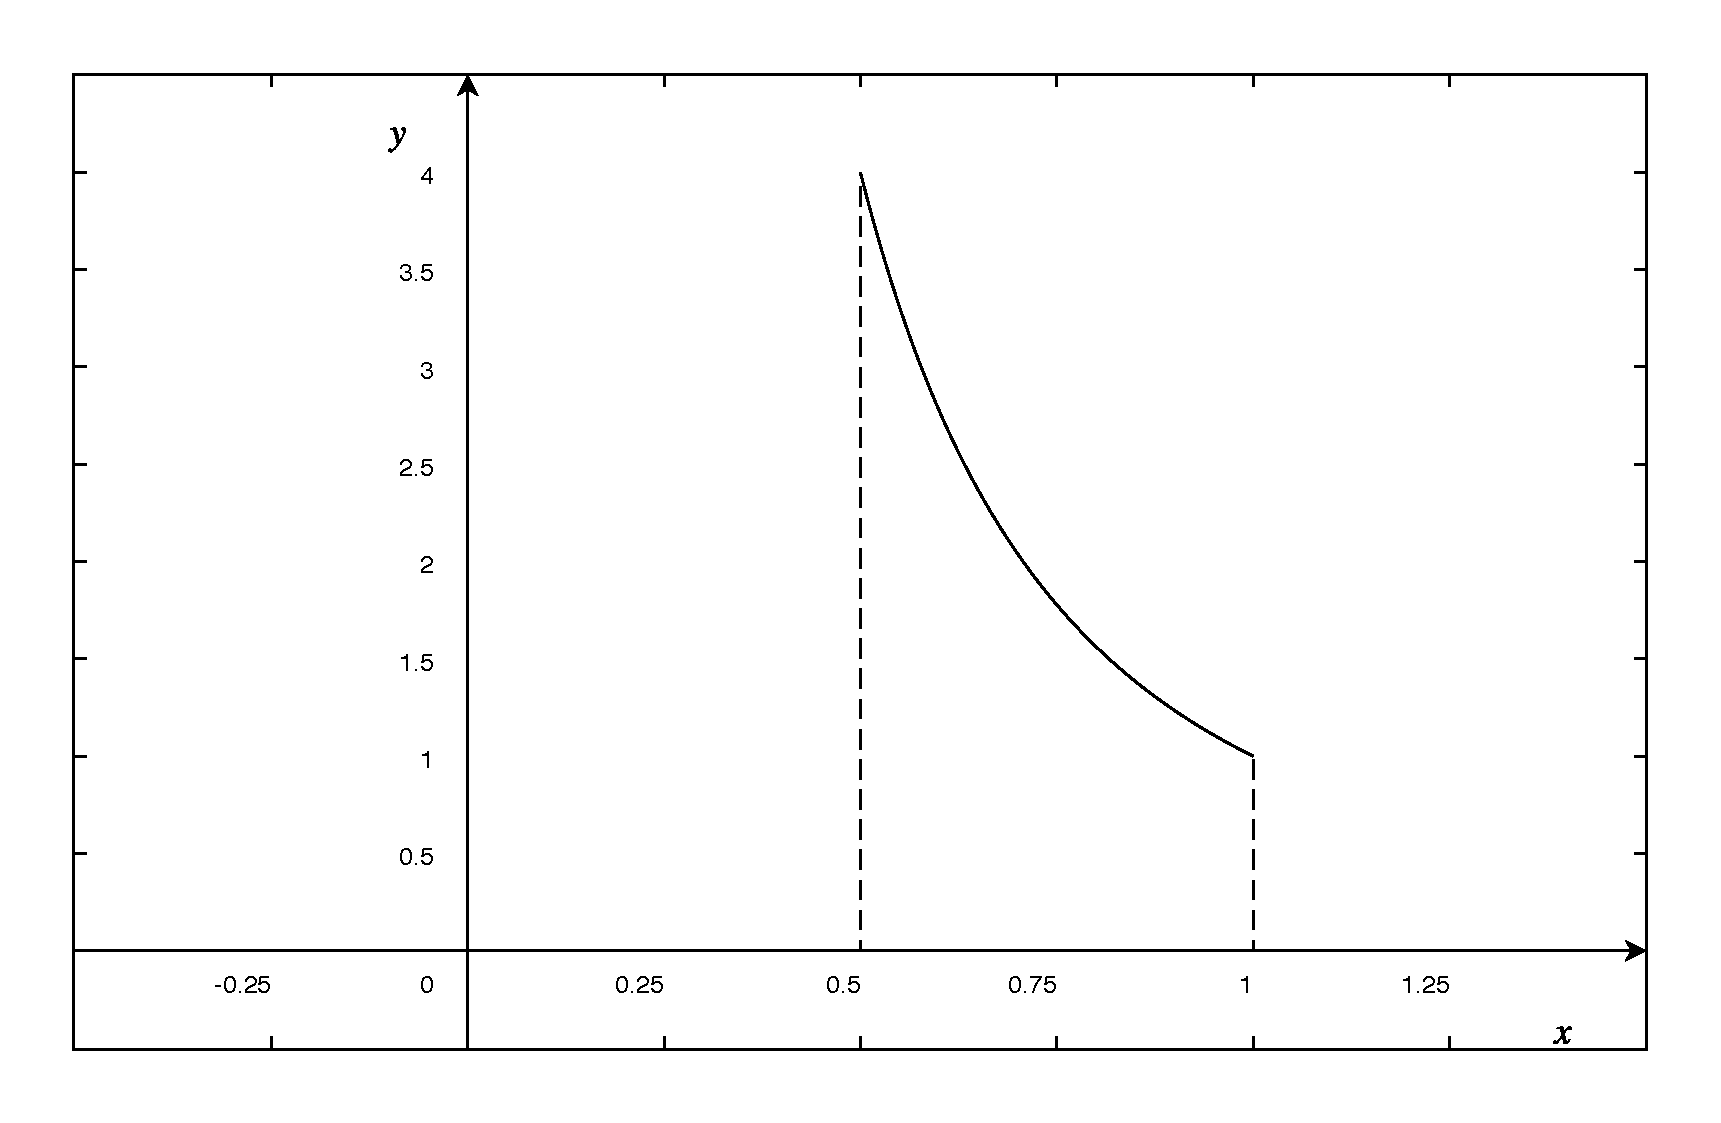
\includegraphics[width=0.5\textwidth]{Figures/Romeo_model_2.pdf}
  \end{figure}
\end{eg}
\begin{remark}[Bayes' rule variant]
  \[
    \mathbb{P}(\theta \vert x_1, x_2) = \dfrac{\mathbb{P}(x_2 \vert \theta, x_1) \mathbb{P}(\theta \vert x_1)}{\mathbb{P}(x_2 \vert x_1)}
  \]
\end{remark}
\begin{proof}
  \[
    \begin{aligned}
      f_{\Theta \vert X_1, X_2} \left(\theta \Big| \dfrac{1}{2}, \dfrac{1}{4}\right) &= \dfrac{f_{\Theta, X_1, X_2} \left(\theta, \dfrac{1}{2}, \dfrac{1}{4}\right)}{f_{X_1, X_2}\left(\dfrac{1}{2}, \dfrac{1}{4}\right)} \\
      &= \dfrac{f_{X_2 \vert \Theta, X_1} \left(\dfrac{1}{4} \Big| \theta, \dfrac{1}{2}\right) f_{\Theta, X_1}\left(\theta, \dfrac{1}{2}\right)}{f_{X_1, X_2}\left(\dfrac{1}{2}, \dfrac{1}{4}\right)} \\
      &= \dfrac{f_{X_2 \vert \Theta, X_1} \left(\dfrac{1}{4} \Big| \theta, \dfrac{1}{2}\right) f_{\Theta \vert X_1}\left(\theta \Big| \dfrac{1}{2}\right) f_{X_1} \left(\dfrac{1}{2}\right)}{f_{X_1, X_2}\left(\dfrac{1}{2}, \dfrac{1}{4}\right)} \\
      &= \dfrac{f_{X_2 \vert \Theta, X_1} \left(\dfrac{1}{4} \Big| \theta, \dfrac{1}{2}\right) f_{\Theta \vert X_1}\left(\theta \Big| \dfrac{1}{2}\right)}{f_{X_2 \vert X_1}\left(\dfrac{1}{4} \Big| \dfrac{1}{2}\right)} \\
    \end{aligned}
  \]
  Thus, 
  \[
    f_{\Theta \vert X_1, X_2} \left(\theta \Big| \dfrac{1}{2}, \dfrac{1}{4}\right) \propto f_{X_2 \vert \Theta, X_1} \left(\dfrac{1}{4} \Big| \theta, \dfrac{1}{2}\right) f_{\Theta \vert X_1}\left(\theta \Big| \dfrac{1}{2}\right)
  \]
\end{proof}

Now it's a bit tedious since we need to perform calculations and adjust our prior each time we obtain new data or observations. However, we also have Bayes's rule for multiple random variables, which simplifies the process. 
\[
  \begin{aligned}
    f_{\Theta \vert X_1, \cdots, X_n} (\theta \vert x_1, \cdots, x_n) &= \dfrac{f_{X_1, \cdots, X_n \vert \Theta} (x_1, \cdots, x_n \vert \theta) f_{\Theta} (\theta)}{Z(x_1, \cdots, x_n)} \\
    &\propto f_{X_1, \cdots, X_n \vert \Theta} (x_1, \cdots, x_n \vert \theta) f_{\Theta} (\theta) \\ 
    &= \underbrace{f_{X_1 \vert \Theta} (x_1 \vert \theta) \cdots f_{X_n  \vert \Theta(x_n \vert \theta)}}_{\text{product of likelihood}} \underbrace{f_{\Theta} (\theta)}_{\text{prior}}
  \end{aligned}
\]
if \(X_1, \cdots, X_n\) are independent given \(\Theta\).  

\begin{eg}[Cont'd]
  Given that Juliet is late by \(\frac{1}{4}\) hours on their third date, how do we find the posterior? 

  \textbf{Solution:} 

  \[
    f_{\Theta \vert X_1, X_2, X_3} \left(\theta \Big| \dfrac{1}{2}, \dfrac{1}{4}, \dfrac{1}{4}\right) \propto f_{X_1 \vert \Theta} \left(\dfrac{1}{2} \Big| \theta\right) f_{X_2 \vert \Theta} \left(\dfrac{1}{4} \Big| \theta\right) f_{X_3 \vert \Theta} \left(\dfrac{1}{4} \Big| \theta\right) f_{\Theta} (\theta) = \dfrac{1}{\theta^3}
  \]

  For \(f_{X_1 \vert \Theta}, f_{X_2 \vert \Theta}, f_{X_3 \vert \Theta}\), they are all equal to \(\frac{1}{\theta}\) for \(\theta \geq \frac{1}{2}\) and \(\theta \geq \frac{1}{4}\) for the same reason shown before. We also have \(f_{\Theta} (\theta) = 1\) if \(0 \leq \theta \leq 1\). Taking the intersection, we obtain \(\frac{1}{\theta^3}\) for \(\frac{1}{2} \leq \theta \leq 1\). For the integral to be equal to 1, we need to determine the constant term, which can be found using calculus.
  \[
    \int_\frac{1}{2} ^1 \dfrac{1}{\theta^2} d \theta = \dfrac{3}{2} \Longrightarrow f_{\Theta \vert X_1, X_2, X_3} \left(\theta \Big| \dfrac{1}{2}, \dfrac{1}{4}, \dfrac{1}{4}\right) = \dfrac{2}{3\theta^3}
  \]  
\end{eg}

\newpage
\begin{eg}[Biased Coin]
  A coin of unknown bias flips HTT. What is the bias?

  \textbf{Solution:} 
  Let \(X \sim \text{Bernoulli}(\Theta)\), where \(\Theta = \mathbb{P}(X = H)\). We have a prior \(\Theta \sim \text{Uniform}(0, 1)\). To find the posterior (bias), we have:
  \[
    \begin{aligned}
      f_{\Theta \vert X_1, X_2, X_3} (\theta \vert H,H,T) &\propto p_{X_1 \vert \Theta} (H \vert \theta) p_{X_2 \vert \Theta} (T \vert \theta) p_{X_3 \vert \Theta} (T \vert \theta) f_{\Theta} (\theta) \\
      &= \theta (1 - \theta) (1 - \theta) \times 1 \\
      &= \theta (1 - \theta)^2 \\
      \Longrightarrow f_{\Theta \vert X_1, X_2, X_3} (\theta \vert H,H,T) &= \dfrac{\theta (1 - \theta)^2}{\int_0 ^1 \theta  (1 - \theta)^2 d \theta} = 12\theta (1 - \theta)^2
    \end{aligned}
  \]
\end{eg}

To find the posterior, we often need to find the denominator \(Z(x)\), which requires some calculus techniques and can sometimes be difficult to solve. However, there are some techniques that come in handy.

\section{Conjugate Priors}

\begin{definition}[Conjugate Priors]
  The posterior distribution \(f_{\Theta \vert X} (\theta \vert x)\) is in the same probability distribution family as the prior distribution \(f_{\Theta} (\theta)\), the prior and posterior are then called conjugate distributions, and the prior is called a conjugate prior for
  the likelihood function\(f_{X \vert \Theta} (x \vert \theta)\).
\end{definition}

There are four types of conjugate priors to consider. 

\subsection{Conjugate Prior for Bernoulli}
\begin{definition}
  Suppose \(X_1, \cdots, X_n\) form a random sample from Bernoulli distribution with an unknown parameter \(\theta\ (0 < \theta < 1)\). If the prior distribution \(f_{\Theta}(\theta)\) is the Beta distribution Beta\((\alpha, \beta)\ (\alpha, \beta > 0)\), then the posterior distribution \(f_{\Theta \vert X}(\theta \vert x)\) given \(\{X_i = x_i\}_i=1^n\) is the Beta distribution Beta\((\alpha + \sum_{i = 1}^n x_i, \beta + n - \sum_{i = 1}^n x_i)\). 
\end{definition}

Here we introduce the Beta random variable. It has the PDF as follows: 
\[
  f_{\Theta} (\theta) = \begin{dcases}
    \dfrac{1}{B(\alpha, \beta)} \theta^{\alpha-1} (1 - \theta)^{\beta - 1} &\text{ for } 0 < \theta < 1 \\
    0 &\text{ otherwise} 
  \end{dcases}, 
\]
where 
\[
  B(\alpha, \beta) = \dfrac{\Gamma(\alpha)\Gamma(\beta)}{\Gamma(\alpha + \beta)}, \quad \Gamma(\alpha) = \int_0^{\infty} x^{\alpha-1} e^{-x} dx = (\alpha - 1)!\ (\text{for positive integer} \alpha)
\]
or equivalently,
\[
  B(\alpha, \beta) = \dfrac{(\alpha - 1)!(\beta - 1)!}{(\alpha + \beta -1)!} .
\]
The reason why \(B(\alpha, \beta)\) appears in the denominator of the PDF is that it serves as the normalization constant, ensuring that the integral equals 1 so that it is a valid PDF.

The Beta random variable is widely used to model the prior distribution of a random variable which range is \([0, 1]\), where \(\alpha\) and \(\beta\) are hyperparameter. 

Recalling the coin flip example above, with the prior \(\Theta\) and observation \(X\) remaining unchanged, we can use the Beta distribution to perform the calculation. We have \(\Theta \sim \text{Uniform}(0, 1) = \text{Beta}(1, 1)\), and for \(h = 1, t = 2\), we have:
\[
  f_{\Theta \vert X_1, X_2, X_3} (\theta \vert H,H,T) = \dfrac{1}{\text{Beta}(h + 1, t + 1)} \theta^{2-1} (1 - \theta)^{3 - 1} = 12\theta (1 - \theta)^2
\]

In general, for a coin of unknown bias flips \(n\) times and gets \(h\) heads and \((n - h)\) tails (or \(t\) tails), we can have prior of \(\Theta \sim \text{Uniform}(0, 1) = \text{Beta}(1, 1)\), and \((\theta \vert h\ \text{heads}, t\ \text{tails}) \sim \text{Beta} (h + 1, t + 1)\). 

\begin{minipage}{0.5\textwidth}
  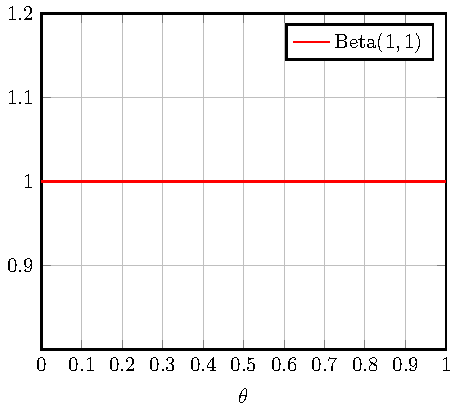
\includegraphics{Figures/Beta_1_1.pdf}
\end{minipage}
\begin{minipage}{0.5\textwidth}
  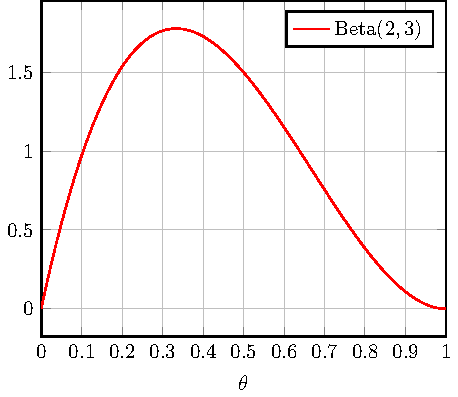
\includegraphics{Figures/Beta_2_3.pdf}
\end{minipage}
\begin{minipage}{0.5\textwidth}
  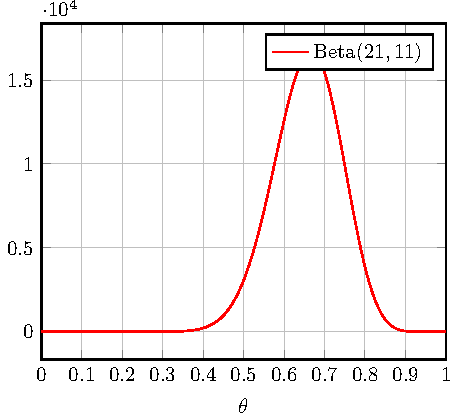
\includegraphics{Figures/Beta_21_11.pdf}
\end{minipage}
\begin{minipage}{0.5\textwidth}
  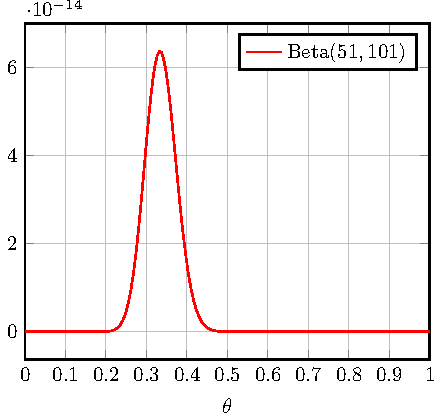
\includegraphics{Figures/Beta_51_101.pdf}
\end{minipage}

The above shows that we can perform estimation based on the number of experiments, which will result in a different PDF.

However, they share a common feature: the value at which the PDF or PMF reaches its maximum is 
\[
  \text{mode}[\theta] = \dfrac{\alpha - 1}{\alpha - 1 + \beta - 1} \quad \text{when}\ \alpha, \beta > 1
\] 

Also, we can treat the different parameters as a change in belief. For example, if Beta(2, 3) is our prior, and we readjust our belief based on observations, we then obtain Beta(21, 11). This shows that the area below the original mode \(\frac{1}{3}\) decreases, making it less probable. 

The last thing to note is that hyperparameter, in the coin flip case, \(h, t\), don’t matter if we observe a large number of data samples, meaning the posterior mainly depends on the observed data. However, if the prior contains a large dataset or the size of the observed data is small, then the prior plays an important role in the posterior. 

\subsection{Conjugate Prior for Poisson}
\begin{definition}
  Suppose \(X_1, \cdots, X_n\) form a random sample from Poisson distribution with an unknown mean \(\Theta > 0\). If the prior distribution \(f_{\Theta}(\theta)\) is the Gamma distribution \(\text{Gamma}(\alpha, \beta)\ (\alpha, \beta >0)\), then the posterior distribution \(f_{\Theta \vert X} (\theta \vert x)\) given \(\{X_i = x_i\}_{i=1} ^n\) is the Gamma distribution \(\text{Gamma}(\alpha + \sum_{i = 1}^n x_i, \beta + n)\). 
\end{definition}

Here we introduce another random variable that is often used as prior, Gamma random variable. It has the PDF as follows: 
\[
  f_{\Theta} (\theta) = \begin{dcases}
    \dfrac{\beta^{\alpha}}{\Gamma (\alpha)}\theta^{\alpha - 1} e^{-\beta\theta} &\text{ for } \theta > 0 \\
    0 &\text{ for } \theta \leq 0 \\
  \end{dcases}, 
\]
where 
\[
  \Gamma (\alpha) = \int_{0}^{\infty} x^{\alpha - 1} e^{-x} dx = (\alpha - 1)!\ (\text{for positive integer}\ \alpha).
\]
Again, we have the Gamma random variable as the denominator because the integral needs to be equal to 1.

\begin{eg}
  At an Apple Store, the number of iPhones sold per day is modeled as a Poisson distribution with unknown mean \(\Theta\). Suppose the prior distribution of \(\Theta\) is Gamma(3, 2). Let \(X\) be the number of iPhones sold in a specific day. If \(X = 3\) is observed, what is the updated distribution of \(\theta\)? 
  
  \textbf{Solution:} 
  Here we have 
  \[
    X \sim \text{Poisson}(\Theta) = \begin{dcases}
      \dfrac{e^{-\theta}\theta^x}{x!} &\text{ for } x = 0, 1, 2 \dots\\
      0  &\text{ otherwise} \\ 
    \end{dcases};
  \]
  \[
    \Theta \sim \text{Gamma}(\alpha, \beta) = \begin{dcases}
      \dfrac{\beta^{\alpha}}{\Gamma (\alpha)}\theta^{\alpha - 1} e^{-\beta\theta} &\text{ for } \theta > 0 \\
      0 &\text{ for } \theta \leq 0 \\
    \end{dcases}.
  \]
  Since we have observed \(X = 3\), 
  \[
    f_{\Theta \vert X} (\theta \vert 3) \propto f_{\Theta} (\theta) f_{X \vert \Theta} (3 \vert \theta)
  \]
  where
  \[
    f_{\Theta} (\theta) = \text{Gamma}(3, 2) = \dfrac{2^3}{2!}\theta^{3-1}e^{-2\theta}, f_{X \vert \Theta} (3 \vert \theta) = \text{Poisson}(\theta) = \dfrac{e^{-\theta}\theta^3}{3!}.
  \]
  Then we have
  \[
    f_{\Theta \vert X} (\theta \vert 3) \propto f_{\Theta} (\theta) f_{X \vert \Theta} (3 \vert \theta) = \dfrac{2^2}{3!} \theta^5 e^{-3\theta} \propto \theta^5 e^{-3\theta}
  \]
  \[
    f_{\Theta \vert X} (\theta \vert 3) = \dfrac{\theta^{6-1} e^{-3\theta}}{Z},\quad Z = \int_{0}^{\infty} \theta^{6-1} e^{-3\theta} d \theta = \dfrac{\Gamma(6)}{3^6}
  \]
  Finally, we have the posterior
  \[
    f_{\Theta \vert X} (\theta \vert 3) = \text{Gamma}(6, 3). 
  \]
\end{eg}

Above is the same as taking \(\alpha = 3, \beta = 2, n = 1 \text{ and } x = 3\), then we have \(\alpha + x = 6\), \(\beta + n = 3\). This directly gives us Gamma(6, 3). 

\subsection{Conjugate Prior for Exponential}
\begin{definition}
  Suppose \(X_1, \cdots, X_n\) form a random sample from Exponential distribution with an unknown parameter \(\theta > 0\). If the prior distribution \(f_{\Theta}(\theta)\) is the Gamma distribution \(\text{Gamma}(\alpha, \beta)\\ (\alpha, \beta > 0)\), then the posterior distribution \(f_{\Theta \vert X} (\theta \vert x)\) given \(\{X_i = x_i\}_{i=1} ^n\) is the Gamma distribution \(\text{Gamma}(\alpha + n, \beta + \sum_{i = 1}^n x_i)\). 
\end{definition}

In the case of Exponential prior, we have \(\alpha =\) no. of trials + 1, \(\beta =\) sum of data \(+\) prior. 

\begin{eg}
  If the number of iPhones sold per hour follows a Poisson distribution with unknown mean \(\Theta\), then the time between two successive iPhones sold follow an exponential distribution with parameter \(\Theta\). Suppose the prior distribution of \(\Theta\) is Gamma(1, 2). Let \(X\) be the time interval (in hour) between successive iPhones sold.

  Assume that we have \(X_1 = 1.5, X_2 = 2, X_3 = 2.5\). 

  \textbf{Solution:} 
  Here we have 
  \[
    X \sim \text{Exponential}(\Theta) = \begin{dcases}
      \theta e^{-\theta x} &\text{ for } x \geq 0 \\
      0  &\text{ for } x < 0 \\ 
    \end{dcases};
  \]
  \[
    \Theta \sim \text{Gamma}(1, 2). 
  \]
  Since we have observed \(X_1, X_2, X_3\), 
  \[
    f_{\Theta \vert X_1, X_2, X_3} (\theta \vert 1.5, 2, 2.5) \propto f_{\Theta} (\theta) f_{X_1, X_2, X_3 \vert \Theta} (1.5, 2, 2.5 \vert \theta)
  \]
  where
  \[
    f_{\Theta} (\theta) = \text{Gamma}(1, 2) = \dfrac{2^1}{1!}\theta^{1-1}e^{-2\theta}, f_{X_1, X_2, X_3 \vert \Theta} (1.5, 2, 2.5 \vert \theta) = (\theta e^{-1.5\theta}) (\theta e^{-2\theta}) (\theta e^{-2.5\theta}). 
  \]
  Then we have
  \[
    f_{\Theta \vert X_1, X_2, X_3} (\theta \vert 1.5, 2, 2.5) \propto f_{\Theta} (\theta) f_{X_1, X_2, X_3 \vert \Theta} (1.5, 2, 2.5 \vert \theta) = 2\theta^3 e^{-(2 + 6)\theta} \propto \theta^3 e^{-(2 + 6)\theta}
  \]
  \[
    f_{\Theta \vert X} (\theta \vert 3) = \dfrac{\theta^3 e^{-(2 + 6)\theta}}{Z},\quad Z = \int_{0}^{\infty} \theta^3 e^{-(2 + 6)\theta} d \theta = \dfrac{\Gamma(4)}{8^4}
  \]
  Finally, we have the posterior
  \[
    f_{\Theta \vert X} (\theta \vert 3) = \text{Gamma}(4, 8). 
  \]
\end{eg}

Above is the same as taking \(\alpha = 1, \beta = 2, n = 3, x_1 = 1.5, x_2 = 2 \text{ and } x_3 = 2.5\), then we have \(\alpha + n = \text{no. of trials} + 1 = 3 + 1= 4\), \(\beta + n = \text{sum of trials} + \text{prior} = 2 + 6 = 8\). This directly gives us Gamma(4, 8). 

\subsection{Conjugate Prior for Normal Distribution}
\begin{definition}
  Suppose \(X_1, \cdots, X_n\) form a random sample from a normal distribution with an unknown mean \(\mu\) and a known variance \(\sigma^2 > 0\). If the prior distribution \(f_{\Theta}(\mu)\) is the normal distribution \(\mathcal{N} (\mu, \sigma_0^2)\), then the posterior distribution \(f_{\Theta \vert X} (\mu \vert x)\) given \(\{X_i = x_i\}_{i=1} ^n\) is the normal distribution \(\mathcal{N}(\mu^{\prime}, \sigma^{\prime2})\), where 
  \[
    \mu^{\prime} = \dfrac{\sigma^2\mu_0 + \sigma_0^2 \sum_{i = 1}^n x_i}{\sigma^2 + n\sigma_0^2} \quad\quad \sigma^{\prime2} = \dfrac{\sigma^2\sigma_o^2}{\sigma^2 + n\sigma_o^2}
  \] 
\end{definition}

\begin{definition}[A more general case]
  Suppose \(X_1, \cdots, X_n\) form a random sample from a normal distribution with a common unknown mean \(\theta\) and the known variance \(\sigma_i^2 > 0\). If the prior distribution \(f_{\Theta}(\theta)\) is the normal distribution \(\mathcal{N} (\mu_0, \sigma_0^2)\), then the posterior distribution \(f_{\Theta \vert X} (\theta \vert x)\) given that \(\{X_i = x_i\}_{i=1} ^n\) is the normal distribution \(\mathcal{N}(\mu, \sigma^2)\), where 
  \[
    \dfrac{\mu}{\sigma^2} = \dfrac{\mu_0}{\sigma_0^2} + \dfrac{x_1}{\sigma_1^2} + \cdots + \dfrac{x_n}{\sigma_n^2} \quad\quad \dfrac{1}{\sigma^2} = \dfrac{1}{\sigma_0^2} + \dfrac{1}{\sigma_1^2} + \cdots + \dfrac{1}{\sigma_n^2}
  \] 
\end{definition}

Here we need to consider a special case when both \(\sigma_0^2\) and \(\sigma^2\) are equal to 1, then we have 
\[
  \mu^{\prime} = \dfrac{\mu_0 + \sum_{i = 1}^n x_i}{1 + n} \quad\quad \sigma^{\prime2} = \dfrac{1}{1 + n}
\]

\begin{eg}
  An \(\mathcal{N}(\Theta, 1)\) random variable takes value 3.97. \(\Theta\) follows a standard normal. What is the posterior of \(\Theta\)?
  
  \textbf{Solution:} 
  Here we have the PDF of \(\mathcal{N} (\mu, \sigma^2)\) 
  \[
    f_X(x) = \dfrac{1}{\sigma \sqrt{2\pi}} e^{-\frac{1}{2}\frac{(x - \mu)^2}{\sigma^2}}
  \]
  Given that the prior = \(\Theta \sim \mathcal{N}(0, 1)\), posterior = \(f_{\Theta \vert X}(\theta \vert x) \propto f_{\Theta} (\theta) f_{X \vert \Theta} (x \vert \theta)\), we have
  \[
    f_{\Theta} (\theta) = \dfrac{1}{\sqrt{2\pi}}e^{-\frac{1}{2}\theta^2} \quad\quad f_{X \vert \Theta} (x \vert \theta) = \dfrac{1}{\sqrt{2\pi}}e^{-\frac{1}{2}(x - \theta)^2}
  \]
  \[
  \begin{aligned}
    f_{\Theta \vert X}(\theta \vert x) \propto f_{\Theta} (\theta) f_{X \vert \Theta} (x \vert \theta) &= \dfrac{1}{\sqrt{2\pi}}e^{-\frac{1}{2}\theta^2} \times \dfrac{1}{\sqrt{2\pi}}e^{-\frac{1}{2}(x - \theta)^2} \\
    &\propto e^{-\frac{1}{2}\theta^2} \times e^{-\frac{1}{2}(x - \theta)^2} \\
    &= e^{-\frac{1}{2}\theta^2 -\frac{1}{2}(x - \theta)^2} \\
    &= e^{-(\sqrt{2}\theta - \frac{1}{\sqrt{2}}x)^2} \underbrace{e^{-\frac{x^2}{4}}}_{\text{constant term}} \\ 
    &\propto e^{-(\sqrt{2}\theta - \frac{1}{\sqrt{2}}x)^2} \\ 
    &= e^{-\frac{1}{2}\frac{(\theta - \frac{x}{2})^2}{(\frac{1}{\sqrt{2}})^2}} \\ 
  \end{aligned}
  \]
  Then we have
  \[
    \mu = \dfrac{x}{2} = \dfrac{3.97}{2} = 1.985 \quad\quad \sigma^2 = (\dfrac{1}{\sqrt{2}})^2 = \dfrac{1}{2}
  \]
  Finally, we have the posterior
  \[
    f_{\Theta \vert X} (\theta \vert 3) = \mathcal{N} (1.985, \dfrac{1}{2})
  \]
\end{eg}

Above is the same as taking \(\mu_0 = 0, x_1 = 3.97, \sigma_0 = 1 \text{ and } \sigma_1 = 1\), then we have 
\[
  \dfrac{1}{\sigma^2} = \dfrac{1}{1} + \dfrac{1}{1} \Longrightarrow \sigma = \dfrac{1}{\sqrt{2}} \quad\quad \dfrac{\mu}{\frac{1}{2}} = \dfrac{0}{1} + \dfrac{3.97}{1} \Longrightarrow \mu = 1.985, 
\]
which directly gives us \(\mathcal{N} (1.985, \dfrac{1}{2})\). 

When \(\sigma_0 = \sigma_1 = \cdots = 1\), we can find \(\sigma\) and \(\mu\) by:
\[
  \sigma = \dfrac{1}{\sqrt{n + 1}}, \quad \mu = \dfrac{x_0 + x_1 + \cdots + x_n}{n + 1}
\] 

\begin{eg}
  Three independent \(\mathcal{N}(\Theta, 1)\) random variables take values 3.97, 4.09, 3.11. What is \(\Theta\)? 
  
  \textbf{Solution:} 
  Here we assume the priors are \(\Theta \sim \mathcal{N} (0, 1)\), and from observation we have \(x_1 = 3.97, x_2 = 4.09, x_3 = 3.11\). 

  Then, for the posterior, we have 
  \[
    f_{\Theta \vert X_1, X_2, X_3} (\theta \vert x_1, x_2, x_3) \sim \mathcal{N} \left(\dfrac{0 + 3.97 + 4.09 + 3.11}{1 + 3}, \left(\dfrac{1}{\sqrt{1 + 3}}\right)^2\right) \approx \mathcal{N} (2.79, \dfrac{1}{4})
  \]
\end{eg}
% L02 finished

\section{Applications of Bayesian Statistic}
In this section, we will study the use of Bayesian Statistics.

To begin with, think about the coin flips event. Assume that you have observed some data, i.e., the first 10 coin flips give the sequence \verb|H T T H T T H T T T|. You now have the model; then, what can it be used for? It turns out that we can use it to make predictions, which tell the probability of the next flip being a head. We can also use it to do estimation, such as determining the probability of heads for this coin. Additionally, we can perform something called hypothesis testing, which helps us find the best guess for the estimation.

\subsection{Prediction} 
Let's revisit the previous dating scenario. 
\begin{eg}
  On her first date, Juliet arrives \(\frac{1}{2}\) hour late. How likely is she to arrive more than \(\frac{3}{4}\) hour late next time? 

  \textbf{Solution:} 
  Let \(X_1, X_2 \sim \text{Uniform}(0, \Theta)\), where \(\Theta = \text{Uniform}(0, 1)\). 
  From the posterior that we calculated before, we have 
  \[
    f_{\Theta \vert X} (\theta \vert \dfrac{1}{2}) = \begin{dcases}
      \dfrac{1}{\theta \ln 2} &\text{ if } \dfrac{1}{2} \leq \theta \leq 1 \\
      0 &\text{ otherwise} 
    \end{dcases}
  \]
  We can then use this posterior to make predictions. 
  \[
    \begin{aligned}
      \mathbb{P}(X_2 \geq \dfrac{3}{4} \vert X_1 = \dfrac{1}{2}) &= \int_{-\infty}^{+\infty} \underbrace{\mathbb{P}\left(X_2 \geq \dfrac{3}{4} \vert X_1 = \dfrac{1}{2}, \Theta = \theta\right) \mathbb{P} \left(\theta \vert X_1 = \dfrac{1}{2}\right)}_{\text{Total Probability Theorems}} d \theta \\
      (*) &= \int_{\frac{1}{2}}^{1} \mathbb{P}\left(X_2 \geq \dfrac{3}{4} \vert X_1 = \dfrac{1}{2}, \Theta = \theta\right) f_{\Theta \vert X} (\theta \vert \dfrac{1}{2}) d \theta \\
      (**) &= \int_{\frac{3}{4}}^{1} \mathbb{P}\left(X_2 \geq \dfrac{3}{4} \vert \Theta = \theta\right) f_{\Theta \vert X} (\theta \vert \dfrac{1}{2}) d \theta \\
      (***) &= \int_{\frac{3}{4}}^{1} (\theta - \dfrac{3}{4}) \dfrac{1}{\theta} \dfrac{1}{\theta \ln 2} d \theta \\
      &= \int_{\frac{3}{4}}^{1} \dfrac{1}{\theta \ln{(2)}} d \theta - \int_{\frac{3}{4}}^{1} \dfrac{3}{4\theta^{2} \ln{(2)}} d \theta \\
      &= \dfrac{\ln \frac{4}{3} - \frac{1}{4}}{\ln 2} \\
      &= 0.054
    \end{aligned}
  \]

  In (*), we change the lower boundary from \(-\infty\) to \(\dfrac{1}{2}\) and the upper boundary from \(+\infty\) to 1 because \(f_{\Theta \vert X} (\theta \vert \dfrac{1}{2})\) would be 0 outside \([\dfrac{1}{2}, 1]\). Then, in (**), we again update the lower boundary to \(\dfrac{3}{4}\) because for \(\dfrac{1}{2} \leq \theta \leq \dfrac{3}{4}\), \(\mathbb{P}(X_2 \geq \dfrac{3}{4} \vert \Theta = \theta)\) would be equal to 0. In (***), we can directly find the left-hand side by \((\theta - \dfrac{3}{4}) \dfrac{1}{\theta}\) because \(X_2 \sim \text{Uniform}(0, \theta)\). The PDF can be directly computed by finding the area.
\end{eg}
\begin{remark}
  One may start with 
  \[
    \int_{-\infty}^{+\infty} \mathbb{P}\left(X_2 \geq \dfrac{3}{4}, \Theta = \theta \vert X_1 = \dfrac{1}{2}\right) d \theta
  \]
  where 
  \[
    \begin{aligned}
      \mathbb{P}\left(X_2 \geq \dfrac{3}{4}, \Theta = \theta \vert X_1 = \dfrac{1}{2}\right) &= \dfrac{\mathbb{P}\left(X_2 \geq \dfrac{3}{4}, \Theta = \theta, X_1 = \dfrac{1}{2}\right)}{\mathbb{P}\left(X_1 = \dfrac{1}{2}\right)} \\
      &= \dfrac{\mathbb{P}\left(X_2 \geq \dfrac{3}{4} \vert X_1 = \dfrac{1}{2}, \Theta = \theta\right)\mathbb{P}\left(X_1 = \dfrac{1}{2}, \Theta = \theta\right)}{\mathbb{P}\left(X_1 = \dfrac{1}{2}\right)} \\
      &= \mathbb{P}\left(X_2 \geq \dfrac{3}{4} \vert X_1 = \dfrac{1}{2}, \Theta = \theta\right) \mathbb{P} \left(\theta \vert X_1 = \dfrac{1}{2}\right)
    \end{aligned}
  \]
\end{remark}

If we have past data and a prior distribution, we can often make predictions.
\begin{eg}
  Assume that we have observed \(n\) heads in coin flips. What is the probability that the next coin flip will also be a head? 
  
  \textbf{Solution:}
  For coin flips, we can use \(X \sim \text{Bernoulli}(\Theta)\), where \(\Theta = \mathbb{P}(X = H)\). So for the prior, we have \(\Theta \sim \text{Uniform}(0, 1) = \text{Beta}(1,1)\). Since the prior follows a beta distribution, the posterior also follows a beta distribution. Therefore, the posterior is given by:
  \[
    \Theta \vert n\ \text{Heads} \sim \text{Beta}(n + 1, 1)
  \]
  \[
    f_{\Theta \vert X_1, \cdots, X_n} (\theta \vert nH) = \dfrac{(n + 1)!}{n!1!}\theta^n = (n + 1)\theta^n
  \]
  We then use this posterior to update our belief, making it the prior for predicting whether the next coin flip will be heads.
  \[
  \begin{aligned}
    \mathbb{P} (H^* \vert nH) &= \int_0^1 \mathbb{P} (H^* \vert \theta) f_{\Theta \vert X_1, \cdots, X_n} (\theta \vert nH) d \Theta \\
    &= \int_0^1 \theta (n + 1)\theta^n d \theta \\\
    &= \dfrac{n + 1}{n + 2}
  \end{aligned}
  \]
  For example, if we have previously flipped \(n = 100\) heads, the probability of the next coin flip being heads is \(\frac{101}{102}\). 
\end{eg}

To summary, in Bayesian prediction, for observation \(X = x\) (past data), if \(X\) is continuous, to predict \(x^* \in [a, b]\) 
\[
  \mathbb{P}(x^* \in [a, b] \vert X = x) = \int_{-\infty}^{+\infty} \mathbb{P}(x^* \in [a, b] \vert \theta) \underbrace{f_{\Theta \vert X} (\theta \vert x)}_{\text{prior}} d \theta
\]
where 
\[
  \mathbb{P}(x^* \in [a, b] \vert \theta) = \int_a^b f_{X \vert \Theta} (x^* \vert \theta) dx^*.
\]
If \(X\) is discrete, then to predict \(x^*\)
\[
  \mathbb{P}(x^* \vert X = x) = \int_{-\infty}^{+\infty} \mathbb{P}(x^* \vert \theta) f_{\Theta \vert X} (\theta \vert x) d \theta 
\] 

\subsection{Point Estimation}
The question then arises: how do we turn the conditional PDF or PMF \(f_{\Theta \vert X} (\theta \vert x)\) estimate into a single number? It turns out we have two methods, namely the Maximum a Posterior (MAP) estimator and the Conditional Expectation (CE) estimator. 

For MAP, we find the most likely value: 
\[
  \theta_{\text{MAP}} = \arg \max_{\theta} f_{\Theta \vert X} (\theta \vert x).
\]

For CE, we find the average among all possible \(\theta\), and the expectation \(\mu = \mathbb{E}[\Theta]\) will minimize the mean square error \(\mathbb{E}[(\Theta - \theta)^2]\): 
\[
  \mathbb{E}[\Theta \vert X = x]. 
\] 

To illustrate, let's return to the dating problem again. 
\begin{eg}
  In Romeo's model, on their first date, Juliet arrived \(\frac{1}{2}\) hour late. What would be his estimate for the probability of Juliet being late?

  \textbf{Solution:} 

  \textbf{MAP (optimistic method)}
  \[
      \text{Posterior } f_{\Theta \vert X} (\theta \vert \frac{1}{2}) = \dfrac{1}{\theta \ln 2}\quad \text{when } \frac{1}{2} \leq \theta \leq 1 \Longrightarrow \arg \max_\theta \dfrac{1}{\theta \ln 2} = \arg \max_\theta \frac{1}{\theta}
  \]
    which gives 
  \[
      \theta_{\text{MAP}} = \frac{1}{2} \quad\quad \text{refers to the \href{page=7}{graph}}
  \]

  \textbf{CE (conservative method)} 
  \[
    \mathbb{E}[\Theta \vert X_1 = \dfrac{1}{2}] = \int_{\frac{1}{2}}^1 \theta \dfrac{1}{\theta \ln 2} d \theta = \dfrac{1}{2\ln 2} \approx0.72
  \]
\end{eg}
\begin{remark}
  Note that prediction refers to forecasting the future value, while estimation involves calculating the likely value of a parameter based on samples.
\end{remark}

Here we have two special cases: 

1. Point estimation for a Beta random variable.

Given that the prior is \(\Theta \sim \text{Beta}(1, 1)\), and the posterior is \(\Theta \vert h \text{ Heads}, t \text{ Tails} \sim \text{Beta}(1 + h, 1 + t)\), where \(\alpha = h + 1, \beta = t + 1\), we have: 
\[
  \text{mode}[\text{Beta}(\alpha, \beta)]: \theta = \dfrac{\alpha - 1}{\alpha - 1 + \beta - 1} \text{ when } \alpha, \beta >1.  
\]
\[
  \theta_{MAP} = \dfrac{\alpha - 1}{\alpha - 1 + \beta - 1} = \dfrac{h}{h + t}
\]
\[
  \text{CE} = \dfrac{\alpha}{\alpha + \beta}
\]
As the number of data points increases, the difference between MAP and CE will become smaller, and we will obtain a closer value. 

2. Point estimation for Normal random variable. 

Given that the prior is \(\Theta \sim \mathcal{N}(\mu_0, 1)\), and the posterior is \(\Theta \vert X_1, \cdots, X_n \sim \mathcal{N} (\frac{\mu_0 + x_1 + \cdots + x_n }{n + 1}, \frac{1}{n + 1})\), we have 
\[
  \text{mode}[\mathcal{N} (\mu, \sigma^2)]: \theta = \mu 
\]
\[
  \theta_{MAP} = \dfrac{\mu_0 + x_1 + \cdots + x_n }{n + 1}
\]
\[
  \text{CE} = \mathbb{E}[\mathcal{N} (\mu, \sigma^2)] = x
\]

\subsection{Hypothesis Testing}
Suppose that in a hypothesis testing problem, \(\Theta\) takes \(m\) values \(\theta_1, \cdots, \theta_m\). Recall that in hypothesis testing, we want to find the best guess for the decision or classification. Then, how do we choose the one for which \(f_{\Theta \vert X} (\theta_i \vert x)\) is the largest (best guess)?

\begin{eg}[Binary hypothesis testing - \(\Theta\) takes two values]~

  Now, you receive an email. It could be spam or legitimate, with \(\Theta = 1\) indicating spam with a 20\% chance, and \(\Theta = 0\) indicating legit with an 80\% chance. Suppose there are two patterns, \(X_1\) and \(X_2\), which are independent given a specific email, to classify whether the email is spam or legit.

  \begin{table}[H]
    \centering
    \begin{tabular}{c|c|c}
        \toprule
        \(\Theta\) & \(\mathbb{P}(X_1 = 1 \vert \theta)\) & \(\mathbb{P}(X_2 = 1 \vert \theta)\)  \\
      \midrule
        \(\Theta = 0\) legit & \(0.03\) & \(0.0001\)  \\
        \(\Theta = 1\) spam & \(0.1\) & \(0.01\)  \\
        \bottomrule
    \end{tabular}
  \end{table}
  Then, in a specific email \(x\), observe that \(X_1 = 1\) and \(X_2 = 0\). Is it spam or legitimate?

  \textbf{Solution:} 
  \[
    \mathbb{P}(\Theta = 1 \vert X_1 = 1, X_2 = 0) \propto \mathbb{P}(X_1 = 1, X_2 = 0 \vert \Theta = 1)\mathbb{P}(\Theta = 1) = 0.1 \times 0.99 \times 0.2 \approx 0.0198
  \]
  \[
    \mathbb{P}(\Theta = 0 \vert X_1 = 1, X_2 = 0) \propto \mathbb{P}(X_1 = 1, X_2 = 0 \vert \Theta = 0)\mathbb{P}(\Theta = 0) = 0.03 \times 0.9900 \times 0.8 \approx 0.0240
  \]
  Thus, MAP \(\Theta = 0\), shows that the email is legitimate. 
\end{eg}

\begin{eg}
  We have two coins, A and B. Coin A has a \(\frac{2}{3}\) probability of landing heads, and coin B has a \(\frac{2}{3}\) probability of landing tails. You flip a random coin and observe the sequence "H H T". Which coin did you flip? What is the probability that you are wrong based on MAP, given the outcome is "H H T"? 

  \textbf{Solution:} 

  Since we have equally likely prior \(\mathbb{P}(\Theta = A) = \mathbb{P}(\Theta = B) = 50\%\), 
  \[
    \begin{aligned}
      \mathbb{P}(\Theta = A \vert HHT) &\propto \mathbb{P}(HHT \vert \Theta = A)\mathbb{P}(\Theta = A) \\
      &= \dfrac{2}{3} \times \dfrac{2}{3} \times \dfrac{1}{3} \times \dfrac{1}{2} = \dfrac{2}{27} \\
      \mathbb{P}(\Theta = B \vert HHT) &\propto \mathbb{P}(HHT \vert \Theta = B)\mathbb{P}(\Theta = B) \\
      &= \dfrac{1}{3} \times \dfrac{1}{3} \times \dfrac{2}{3} \times \dfrac{1}{2} = \dfrac{1}{27} \\
    \end{aligned}
  \]
  Thus, MAP \(\Theta = A\). 
  \[
    \begin{aligned}
      \text{error} &= \mathbb{P}(B \vert HHT) \\
      &= \dfrac{\mathbb{P}(HHT \vert \Theta = B) \mathbb{P}(\Theta = B)}{\mathbb{P}(HHT)} \\
      &= \dfrac{\frac{1}{27}}{\frac{1}{27} + \frac{2}{27}} \\
      &= \dfrac{1}{3}
    \end{aligned}
  \]
  This shows that the event would be wrong at \(\frac{1}{3}\) of the time. 
\end{eg}

We find the probability that, even if the calculation is correct, it is still possible for us to make a wrong guess from time to time. But then, what is the probability of being wrong on average? 

% L03 finished
% END OF DOCUMENT